\documentclass[a4,paper,fleqn]{article}

\usepackage{layout}

\newcommand{\uuline}[1]{{\underline{\underline{#1}}}}

\title{AES - Übung 3}
\date{10. März 2016}
\author{Markus Birrer \\
        Yannick Inderbitzin\\
        Daniel Winz}

\begin{document}
\maketitle
%\clearpage
\vfill
\tableofcontents
\vfill
\clearpage

\section{Kurzfragen}
\begin{itemize}
\item Wie ist die Energie- und Leistungsdichte eines SCAPs definiert? \\
    \[ E' = \frac{1}{2 \cdot m} \cdot C \cdot {U_{SCAP_{max}}}^{2} \]
    \[ P' = \frac{U_{SCAP_{max}} \cdot I}{m} 
    = \frac{U_{SCAP{_{max}}}}{\left(R_{S} + R_{L}\right) \cdot m} 
    \cdot \frac{U_{SCAP_{max}}}{2} 
    = \uuline{\frac{{U_{SCAP_{max}}}^{2}}{4 \cdot R_{S} \cdot m}} \]
\item Wie gross ist eine SCAP-Zeitkonstante typisch? Was last sich davon 
ableiten? \\
    Im Bereich von $1\si{\second}$ ($\tau = R_{i} \cdot C$)
\item Was lässt sich über den Wirkungsgrad von SCAPs generell aussagen? Wie 
gross ist er bezogen auf die Leistung, die durch die 
Leistungsdichte-Definition gegeben ist. Kommentar? \\
    Wirkungsgrad: 0.85 \ldots 0.98 \\
    Die Leistungsdichte ist sehr hoch, die Energiedichte hingegen ist gering. \\
    Bei starker Belastung (Lade-/Entladezeit) sinkt der Wirkungsgrad massiv 
    (0-0.5) \\
\item Wann macht die Kombination von Supercaps und Batterien Sinn? Was gilt es 
bei der Kombination von Supercaps und Batterien zu beachten? \\
    Die Kombination von Batterie und Supercap macht Sinn, wenn sowohl während 
    langer Zeit Leistung benötigt wird (Energie = Akku) und gleichzeitig 
    starke Schwankungen in der Leistung vorhanden sind (Leistung = Supercap)
\item Gibt es Unterschiede bei der Integration von Supercaps gegenüber 
Batterien? \\
    Ja, Supercaps verhalten sich anders als Batterien, u.a. Leistungsdichte 
    und Entladung. Dies muss bei der Integration in Betracht gezogen werden. 
    z.B. dickere Leitungen für Supercaps oder auch ein anderes, angepasstes 
    Energiemanagement-System. Auch der Ausgleich der Zellen muss im Auge 
    behalten werden.
\end{itemize}

\clearpage
\section{Berechnung LiIonen Batterien als Vergleich}
\begin{itemize}
\item Berechnen Sie die Energiedichte. \\
    $80\si{\watt\hour\per\kilogram}$ \\
    pro Zelle zu 365\si{\gram} $\Rightarrow$ 29.2\si{\watt\hour\per Zelle}
\item Berechnen Sie die Leistungsdichte der Ladung und der Entladung. 
Kommentare? \\
    \[ P = \frac{U \cdot I}{m} \]
    Ladung: 
    \[ \frac{3.2\si{\volt} \cdot 30\si{\ampere}}{0.365\si{\kilogram}} = 263 \si{\watt\per\kilogram} \]
    Entladung: 
    \[ \frac{3.2\si{\volt} \cdot 100\si{\ampere}}{0.365\si{\kilogram}} = 876.7 \si{\watt\per\kilogram} \]
\item  Berechnen Sie den Wirkungsgrad für nur eine 10C Entladung und separat 
nur für eine 3C Ladung.  Berechnen Sie den Gesamtwirkungsgrad für den 
gesamten Zyklus (Entladung und Ladung).  Annahme: Nur CC Ladeverfahren für 
den ganzen Energieinhalt. \\
    Wirkungsgrad für 10C Entladung $\to$ 100\si{\ampere}: 
    \[ R_{tot} = \frac{U}{I} = \frac{3.2\si{\volt}}{100\si{\ampere}} 
    = 0.032\si{\ohm} \]
    \[ R_s = 0.005\si{\ohm} \Rightarrow R_L 
    = R_{tot} - R_S = 0.032\si{\ohm} - 0.005\si{\ohm} = 0.027\si{\ohm} \]
    \[ \eta_1 = \frac{R_L}{R_L + R_S} = \frac{0.027}{0.032} = 0.843 \]
    Wirkungsgrad für 3C Ladung $\to$ 30\si{\ampere}: 
    \[ R_{tot} = \frac{U}{I} = \frac{3.65\si{\volt}}{30\si{\ampere}} 
    = 0.121\si{\ohm} \]
    \[ R_s = 0.005\si{\ohm} \Rightarrow R_L 
    = R_{tot} - R_S = 0.121\si{\ohm} - 0.005\si{\ohm} = 0.116\si{\ohm} \]
    \[ \eta_2 = \frac{R_L}{R_L + R_S} = \frac{0.116}{0.121} = 0.958 \]
    Gesamtwirkungsgrad für gesamten Zyklus (Entladung und Ladung) nur CC: \\
    \[ \eta_{tot} = \eta_1 \cdot \eta_2 = 0.843 \cdot 0.958 
    = 0.808 \Rightarrow 80.8\% \]
\end{itemize}

\clearpage
\section{Messung Supercaps}
\subsection{Bestimmung Innenwiderstand}
Zunächst wird der SCAP auf eine Spannung von 2.7\si{\volt} aufgeladen. Dazu 
wird beim ein maximaler Strom von 30\si{\ampere} eingestellt. Die Ladung 
erfolgt zunächst als Konstantstromladung (CC). Nach dem Erreichen der 
Ladeschlussspannung wird der Ladevorgang als Konstantspannungsladung (CV) 
fortgesetzt. 

\begin{figure}[h!]
    \centering
    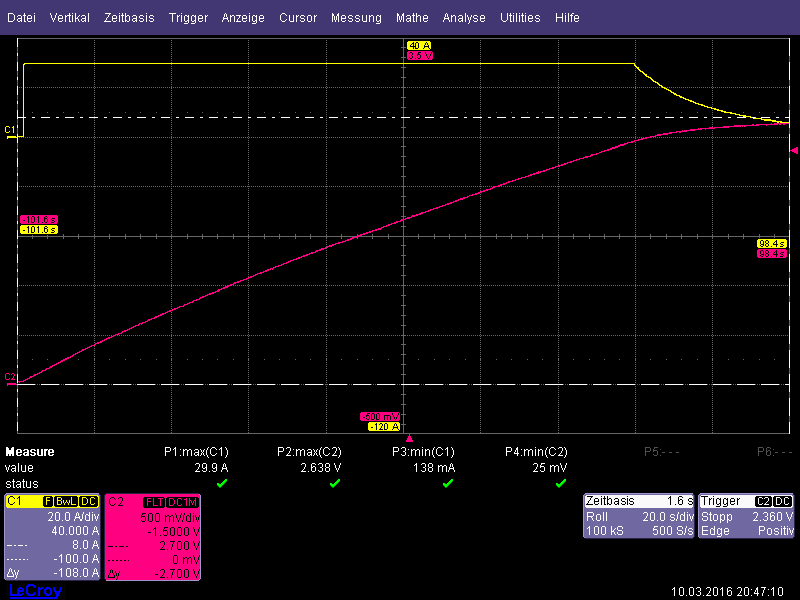
\includegraphics[width=0.7\textwidth, trim=0 20 0 45, clip=true]{fig/charge.png}
    \caption{Ladevorgang $\to$ 30\si{\ampere}}
    \label{fig:charge}
\end{figure}

\noindent
Anschliessend wird der SCAP zur Bestimmung des Innenwiderstandes mit einem 
Strom vom 100\si{\ampere} entladen. Dabei wird die Spannung des SCAP gemessen. 
Aus dem Spannungsabfall nach dem Einschalten der Last kann der Innenwiderstand 
berechnet werden. 

\begin{figure}[h!]
    \centering
    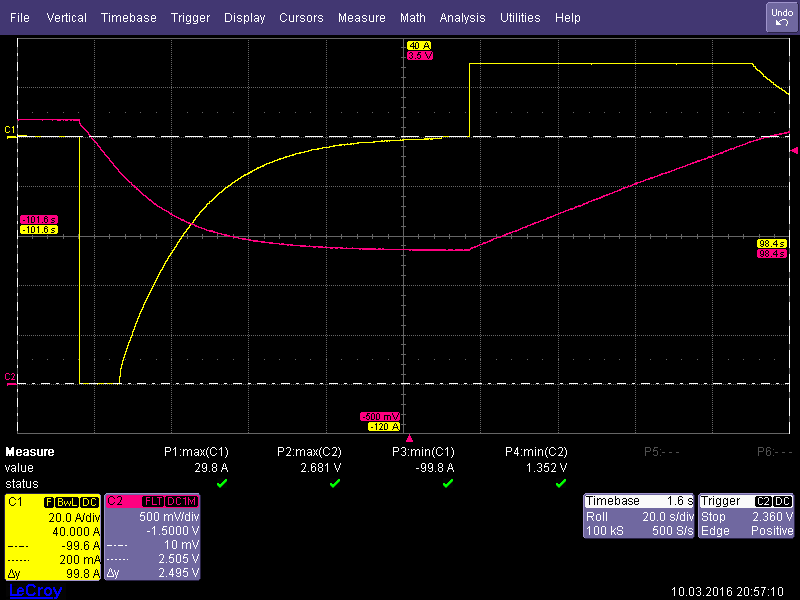
\includegraphics[width=0.7\textwidth, trim=0 20 0 45, clip=true]{fig/discharge2.png}
    \caption{Endladevorgang $\to$ $\Delta I = 100 \si{\ampere}$}
    \label{fig:discharge_i}
\end{figure}

\begin{figure}[h!]
    \centering
    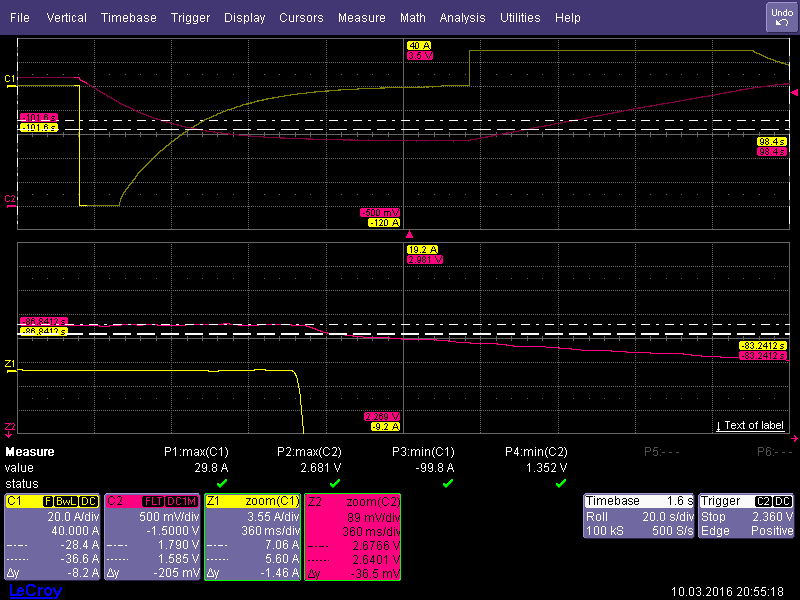
\includegraphics[width=0.7\textwidth, trim=0 20 0 45, clip=true]{fig/discharge1.png}
    \caption{Spannungsverlauf zu Begin des Endladevorgangs $\to$ $\Delta U = 36.5\si{\milli\volt}$}
    \label{fig:discharge_u}
\end{figure}

\[ R_i = \frac{\Delta U}{\Delta I} 
= \frac{36.5\si{\milli\volt}}{100\si{\ampere}} = 0.365\si{\milli\ohm} \]

\clearpage
\subsection{Messung Kurzschluss}
\begin{figure}[h!]
    \centering
    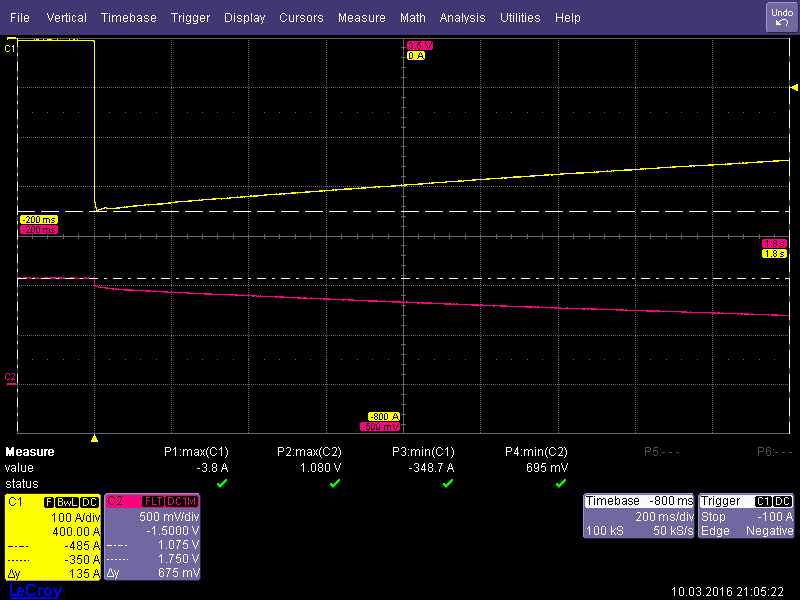
\includegraphics[width=0.7\textwidth, trim=0 20 0 45, clip=true]{fig/short1.png}
    \caption{Kurzschlussversuch}
    \label{fig:short}
\end{figure}

\[ R_i = \frac{\Delta U}{\Delta I} 
= \frac{75\si{\milli\volt}}{350\si{\ampere}} = 0.214\si{\milli\ohm} \]
\[ R_L = \frac{U}{I} = \frac{1\si{\volt}}{350\si{\ampere}} 
= 2.857\si{\milli\ohm} \]

\subsection{Schlussdiskussion}
Der Innenwiderstand beträgt gemäss Datenblatt 0.35\si{\milli\ohm}. Der 
gemessene Wert von 0.365\si{\milli\ohm} liegt sehr nahe an diesem Wert. Der 
gemessene Innenwiderstand der Kurzschlussmessung liegt deutlich tiefer. Dies 
ist jedoch auf die geringe Auflösung der Kondensatorspannung zurückzuführen. 
Wie die Messungen zeigen, liegt der Lastwiderstand beim Kurzschlussversuch 
ungefähr um den Faktor 10 über dem Innenwiderstand des SCAP. Damit liegt keine 
Leistungsanpassung vor. 

\clearpage
\section{Bewertungsbeispiel Akkubohrer}
In dieser Aufgabe soll gezeigt werden, ob ein SCAP-Speicher für eine 
elektrische Akkubohrmaschine eine mögliche Alternative ist. Die Vorteile wären 
klar die schnellere Aufladung des Speichers, sowie der geringere Verschleiss, 
bzw. die längere Lebensdauer des Speichers. Es soll ein handelsüblicher 
Akkubohr-Akku mit 16 \si{\watt\hour} durch einen SCAP-Speicher ersetzt werden.

\subsection{Bestimmung des Speichers}
Als erstes kann die benötigte Kapazität mit der Formel 
\[ E=\frac{1}{2} \cdot C \cdot \left({U_{max}}^2-{U_{min}}^2\right) \]
berechnet werden. Dies ergibt bei einer Maximalspannung von 13\si{\volt} und 
einer Minimalspannung von 5.5\si{\volt} eine Kapazität von 830\si{\farad}. Nun 
kann die Anzahl benötigter SCAPs bestimmt werden. Die Maximalspannung ist mit 
13\si{\volt} vorgegeben, bei einer maximalen Zellspannung von 2.7\si{\volt} 
müssen 5 SCAPs in Serie geschaltet werden um die Maximalspannung zu erreichen. 
Die Kapazität eines Seriestranges kann mit obiger Formel berechnet werden und 
beträgt 400\si{\farad}. Um die erforderliche Kapazität zu erreichen wird ein 
zweiter Seriestrang parallel zum ersten geschaltet. Somit wird eine Kapazität 
von 800\si{\farad} erreicht, die annähernd der berechneten 830\si{\farad} 
entsprechen.
Der so bestimmte SCAP-Speicher sieht wie folgt aus:
\begin{figure}[h!]
    \centering
    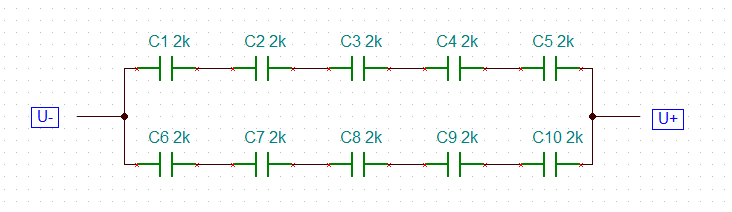
\includegraphics[width=0.8\textwidth]{fig/schema.png}
    \caption{Schema des SCAP Speichers}
    \label{fig:schematic}
\end{figure}

\noindent
\begin{zebratabular}{@{}lll}
\rowcolor{gray} \multicolumn{3}{@{}l}{Die gesuchten Daten} \\
    Gewicht:            
        & $10 \cdot 0.365\si{\kilogram}$              
        & = 3.65\si{\kilogram} \\
    Preis:              
        & $10 \cdot 50\text{Fr}$                    
        & = 500\text{Fr} \\
    DC-Innenwiderstand: 
        & $\frac{5 \cdot 0.35\si{\milli\ohm}}{2}$  
        & = 0.875\si{\milli\ohm} \\
    Volumen:            
        & $10 \cdot 1\si{\deci\metre} \cdot {(0.6\si{\deci\metre})}^2$          
        & = 3.6\si{\litre} \\
\end{zebratabular}

\clearpage
\subsection{Diskussion}
Der bestimmte SCAP-Speicher erreicht mit 15.41\si{\watt\hour} annähernd die 
gewünschte Grösse von 16\si{\watt\hour}. Bedenkt man jedoch, dass die 
Maximalspannung bei fünf in Serie geschalteten SCAPs bei 13.5\si{\volt} liegt, 
wird ein Wert von 16.88\si{\watt\hour} erreicht. Der Speicher ist so in der 
Lage die erforderliche Energie zur Verfügung zu stellen. Der Speicher kann so 
wesentlich schneller geladen werden, als ein üblicher Akku. Auch der sehr 
niedrige Innenwiderstand von rund 0.9\si{\milli\ohm} ermöglicht ein 
verlustarmes Laden des Speichers.

\noindent
Das Gewicht des Speichers von 3.6\si{\kilogram} ist jedoch sehr hoch, und in 
der Praxis wohl nicht anwendbar. Auch wenn man den Speicher halbiert und nur 
ein Seriestrang verwendet, kann das in der Aufgabe beschriebene 
Lastprofil noch bewältigt werden. Bei dieser Lösung wäre das Gewicht von 
1.5\si{\kilogram} immer noch zu hoch. Ausserdem ist der Preis mit 500.- Fr. 
für einen SCAP-Speicher im Vergleich zu einem handelsüblichen Akku viel zu 
hoch. Nicht zuletzt ist auch das benötigte Volumen von 3.6 Litern viel grösser 
als das eines Akkus. Bedenkt man ausserdem die Position des Speichers bei 
einem Akkubohrer wird klar, dass das Werkzeug nicht mehr mit nur einer Hand 
gehalten werden kann, da der Speicher sowohl volumenmässig als auch der aus 
dem Gewicht resultierenden Hebel zu gross würde.

\noindent
Abschliessend kann gesagt werden, dass ein SCAP-Speicher für einen Akkubohrer 
elektrotechnisch möglich wäre. Aus praktischer und finanzieller Sicht ist er 
jedoch zum aktuellen Zeitpunkt nicht sinnvoll.

\end{document}
